\documentclass[
  a4paper,
  12pt,
  english,
  brazilian,
]{article}

\usepackage{pdflscape}
\usepackage{pdfpages}
\usepackage[]{fatec-article}

\begin{document}
\vspace{8cm}
\begin{center}
    \large \textbf{\title{ARTEFATOS DO PROJETO DE SOFTWARE - CRIAÇÃO DE CAMARÃO EM CATIVEIRO COM MONITORAMENTO IOT PARA GASTRONOMIA}}
\end{center}

\maketitle

\break

\tableofcontents

\break



\section*{Diagramas UML}
    Nesta seção serão apresentados os diagramas da UML utilizados para a modelagem do sistema desenvolvido. Dentre os diagramas utilizados, pode-se citar: Diagrama de Caso de Uso e Diagrama de Redes.
    
    \subsection*{\textbf{Diagrama de Caso de Uso}}
    \addcontentsline{toc}{section}{Diagrama de Caso de Uso}

    O Diagrama de Caso de Uso foi desenvolvido para demonstrar as funcionalidades do sistema. O Carcinicultor irá fornecer ao Sistema suas informações para realizar o cadastro/login e o sistema deverá fornecer a tela inicial. Dentro do sistema, o carcinicultor deverá editar dados referentes ao tanque e do sítio em que estão os tanques. Além disso, o sistema fornecerá ao carcinicultor o relatório geral e individual de cada um dos tanques que irá contar com temperatura, pH e amônia.

    Enquanto o carcinicultor utilizar o sistema, ele receberá notificações a respeito dos tanques e dos camarões, verificar informações o sítio e de seu peril.

\begin{figure}[!h]
\centering
\caption{Diagrama de caso de uso}%
\label{fig:diagrama-caso-uso}
 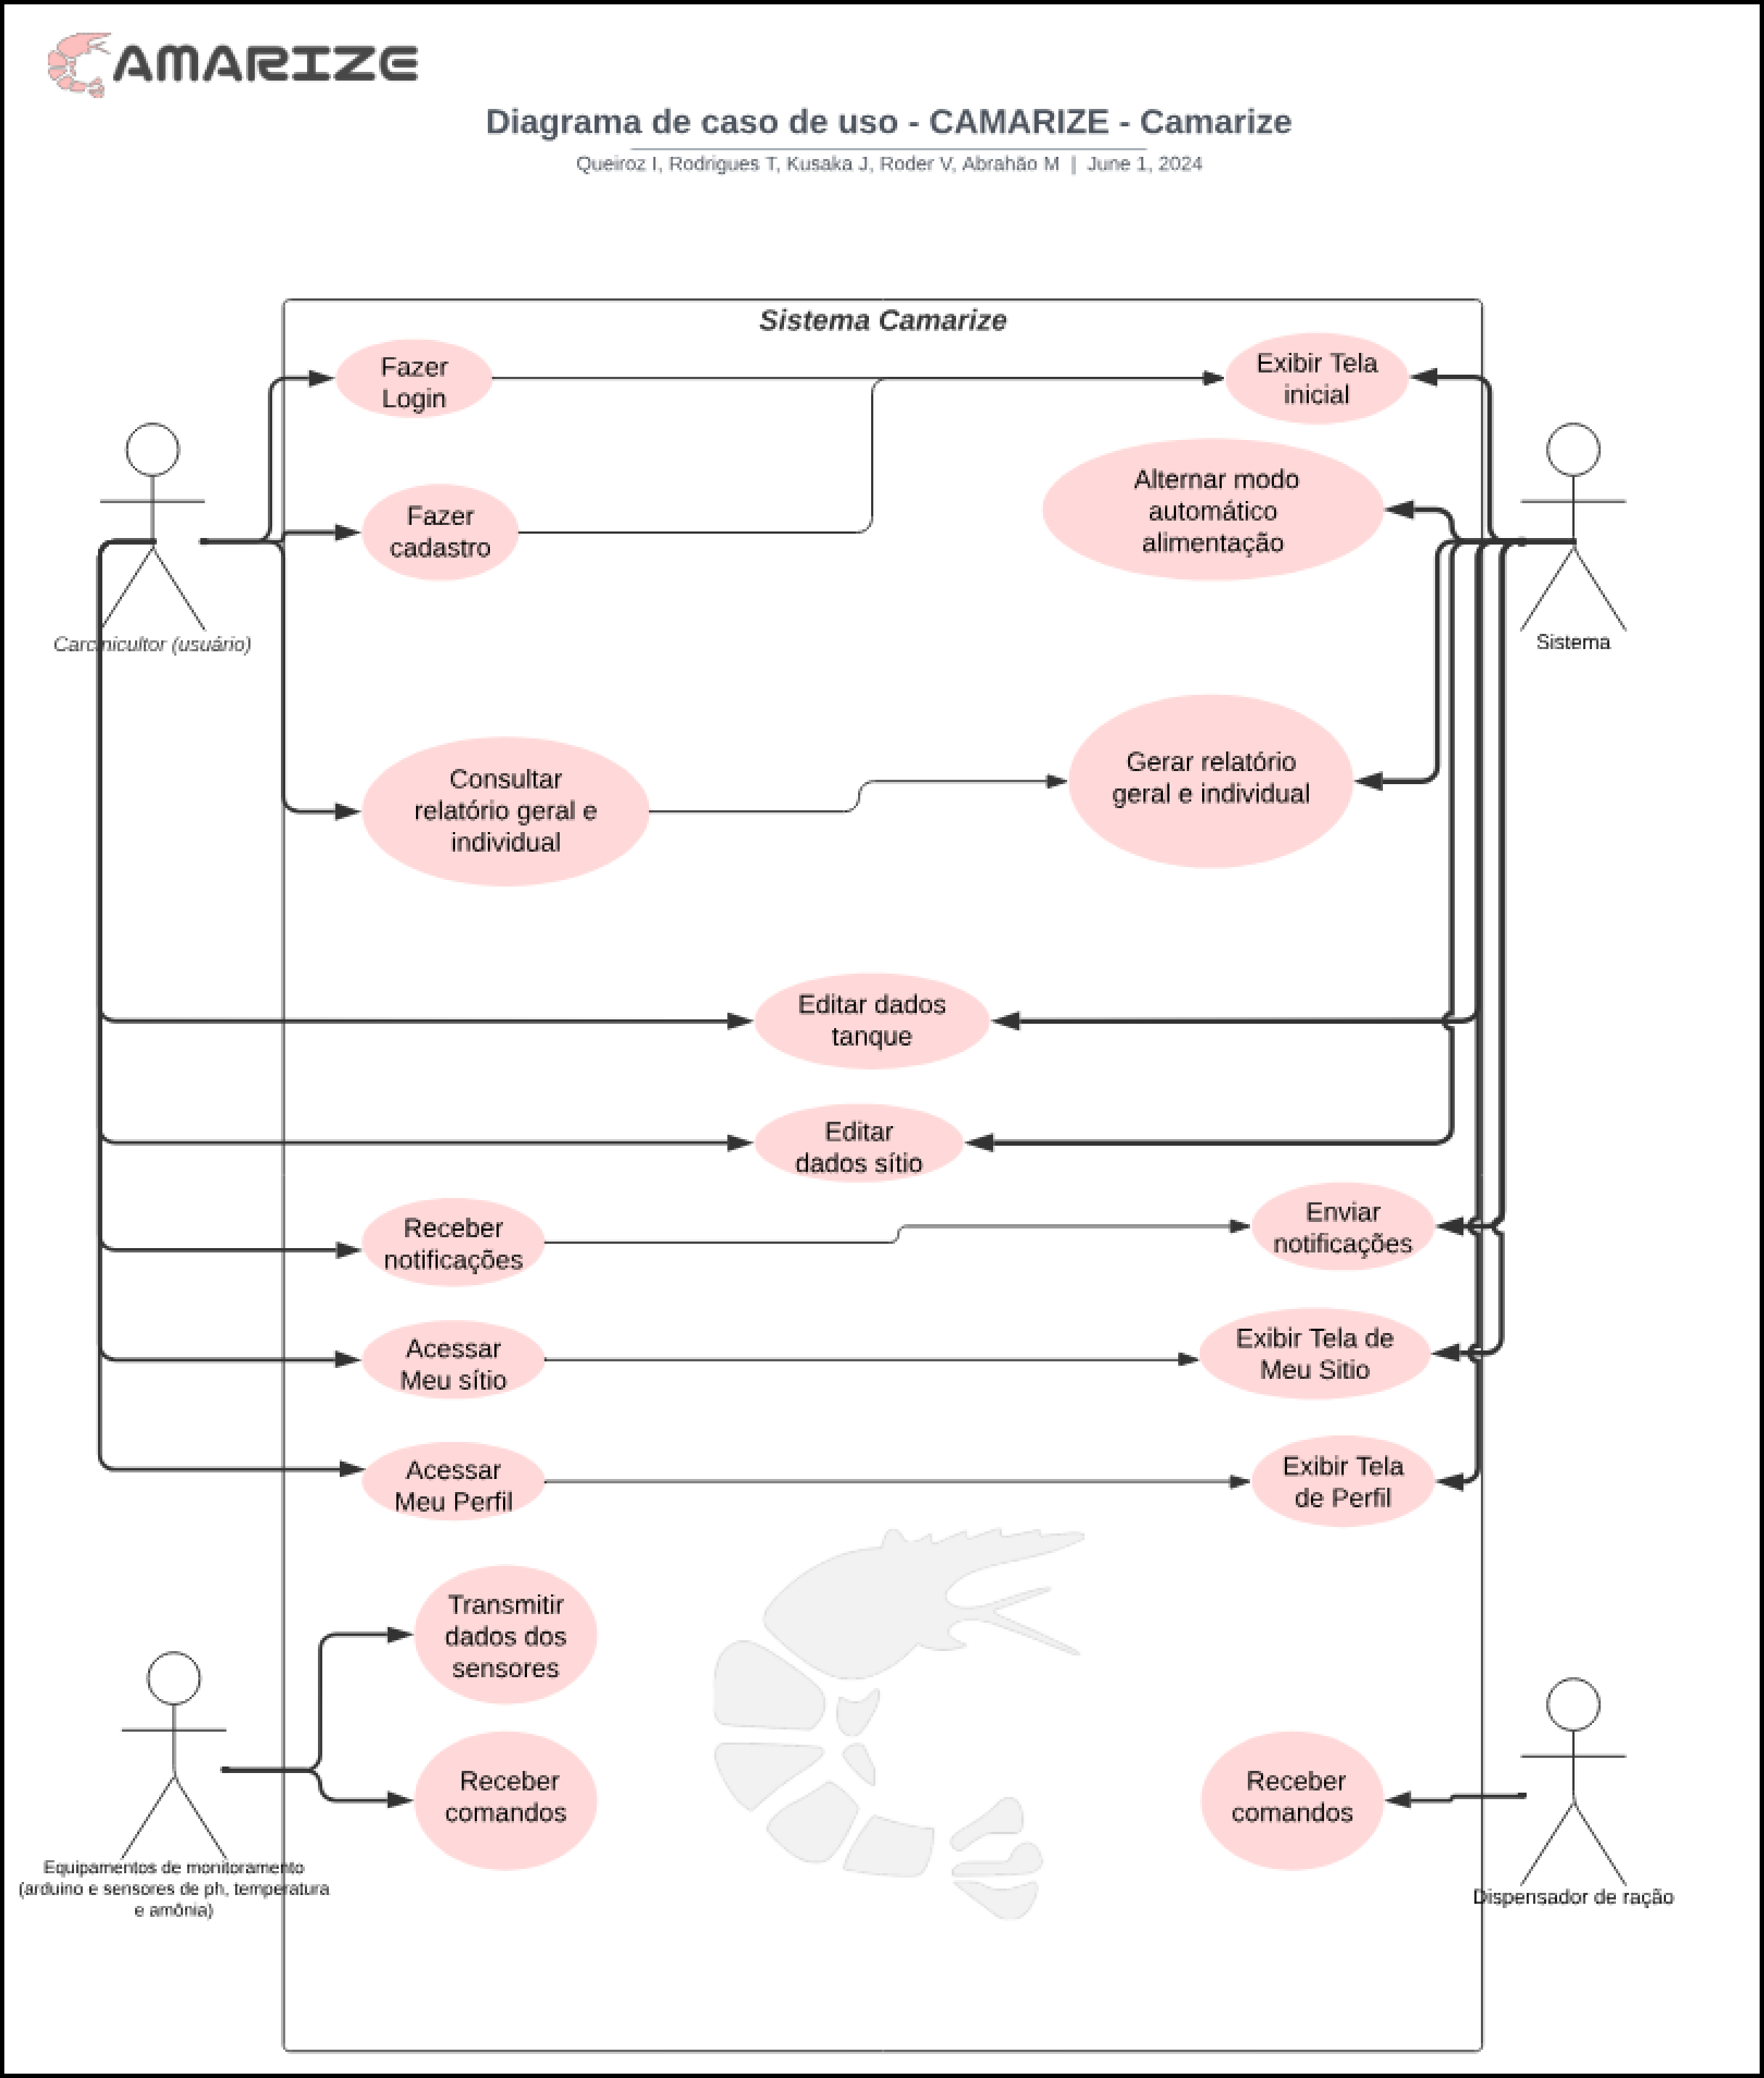
\includegraphics[width=0.8\textwidth]{Imagem/Caso de Uso.png}
\SourceOrNote{Autoria Própria}
\end{figure}

    \newpage
    
    Os equipamentos de monitoramento irão transmitir os dados de cada sensor e receberão comandos. O dispensador de ração irá receber o comando para liberar a ração para os camarões

    \newpage

    \subsection*{\textbf{Diagrama de Classe}}
    \addcontentsline{toc}{section}{Diagrama de Classe}

O diagrama de classes define a estrutura e os relacionamentos necessários para monitorar e otimizar as condições de criação de camarões. Ele inclui classes e associações projetadas para gerenciar dietas, parâmetros ambientais, tipos de camarão e sensores, garantindo operações eficientes e integradas.

Entre as principais classes, Tipos\_camarao categoriza espécies de camarões por meio de um identificador único e um nome. Dietas gerencia as alimentações ideais para cada espécie, enquanto Condições\_ideais define parâmetros ambientais recomendados, como temperatura, pH e amônia, associados a cada tipo de camarão. Parâmetros\_atuais registra as condições ambientais em tempo real de cada cativeiro, e Especif\_camarao conecta condições ideais às dietas recomendadas. Já Cativeiros representa as instalações de criação, relacionando aos tipos de camarão e armazenando dados como médias diárias de temperatura e pH.

O sistema também inclui classes como Alimentação, que documenta horários e detalhes nutricionais, vinculando as dietas aos cativeiros. Sítios registra informações sobre locais onde estão os cativeiros, enquanto Sensores monitoram dados ambientais e estão associados aos cativeiros. Usuários gerenciam o sistema por meio de autenticação e dados pessoais, e os relatórios individuais e gerais detalham os desempenhos dos cativeiros com base nos dados coletados.

Os relacionamentos são fundamentais no sistema. Por exemplo, cada cativeiro está associado a um único tipo de camarão, enquanto um tipo de camarão pode estar ligado a vários cativeiros. Os Parâmetros\_atuais monitoram condições específicas de cativeiros, e a alimentação é registrada de forma vinculada a dietas e cativeiros específicos. Além disso, Sítios podem agregar múltiplos cativeiros, enquanto os sensores mapeiam as condições de cativeiros individuais. Usuários gerenciam sítios específicos e recebem notificações com recomendações baseadas nos dados monitorados.

O uso de multiplicidade (como 1..*, 0..1) garante a flexibilidade e consistência dos relacionamentos, permitindo que o sistema opere de forma robusta e organizada. Este diagrama reflete um design completo, garantindo o monitoramento eficiente das condições ambientais, o controle das dietas e o gerenciamento dos cativeiros de camarões.

    \begin{figure}[!h]
        \centering
        \caption{Diagrama de classe}%
        \label{fig:diagrama-classe}
         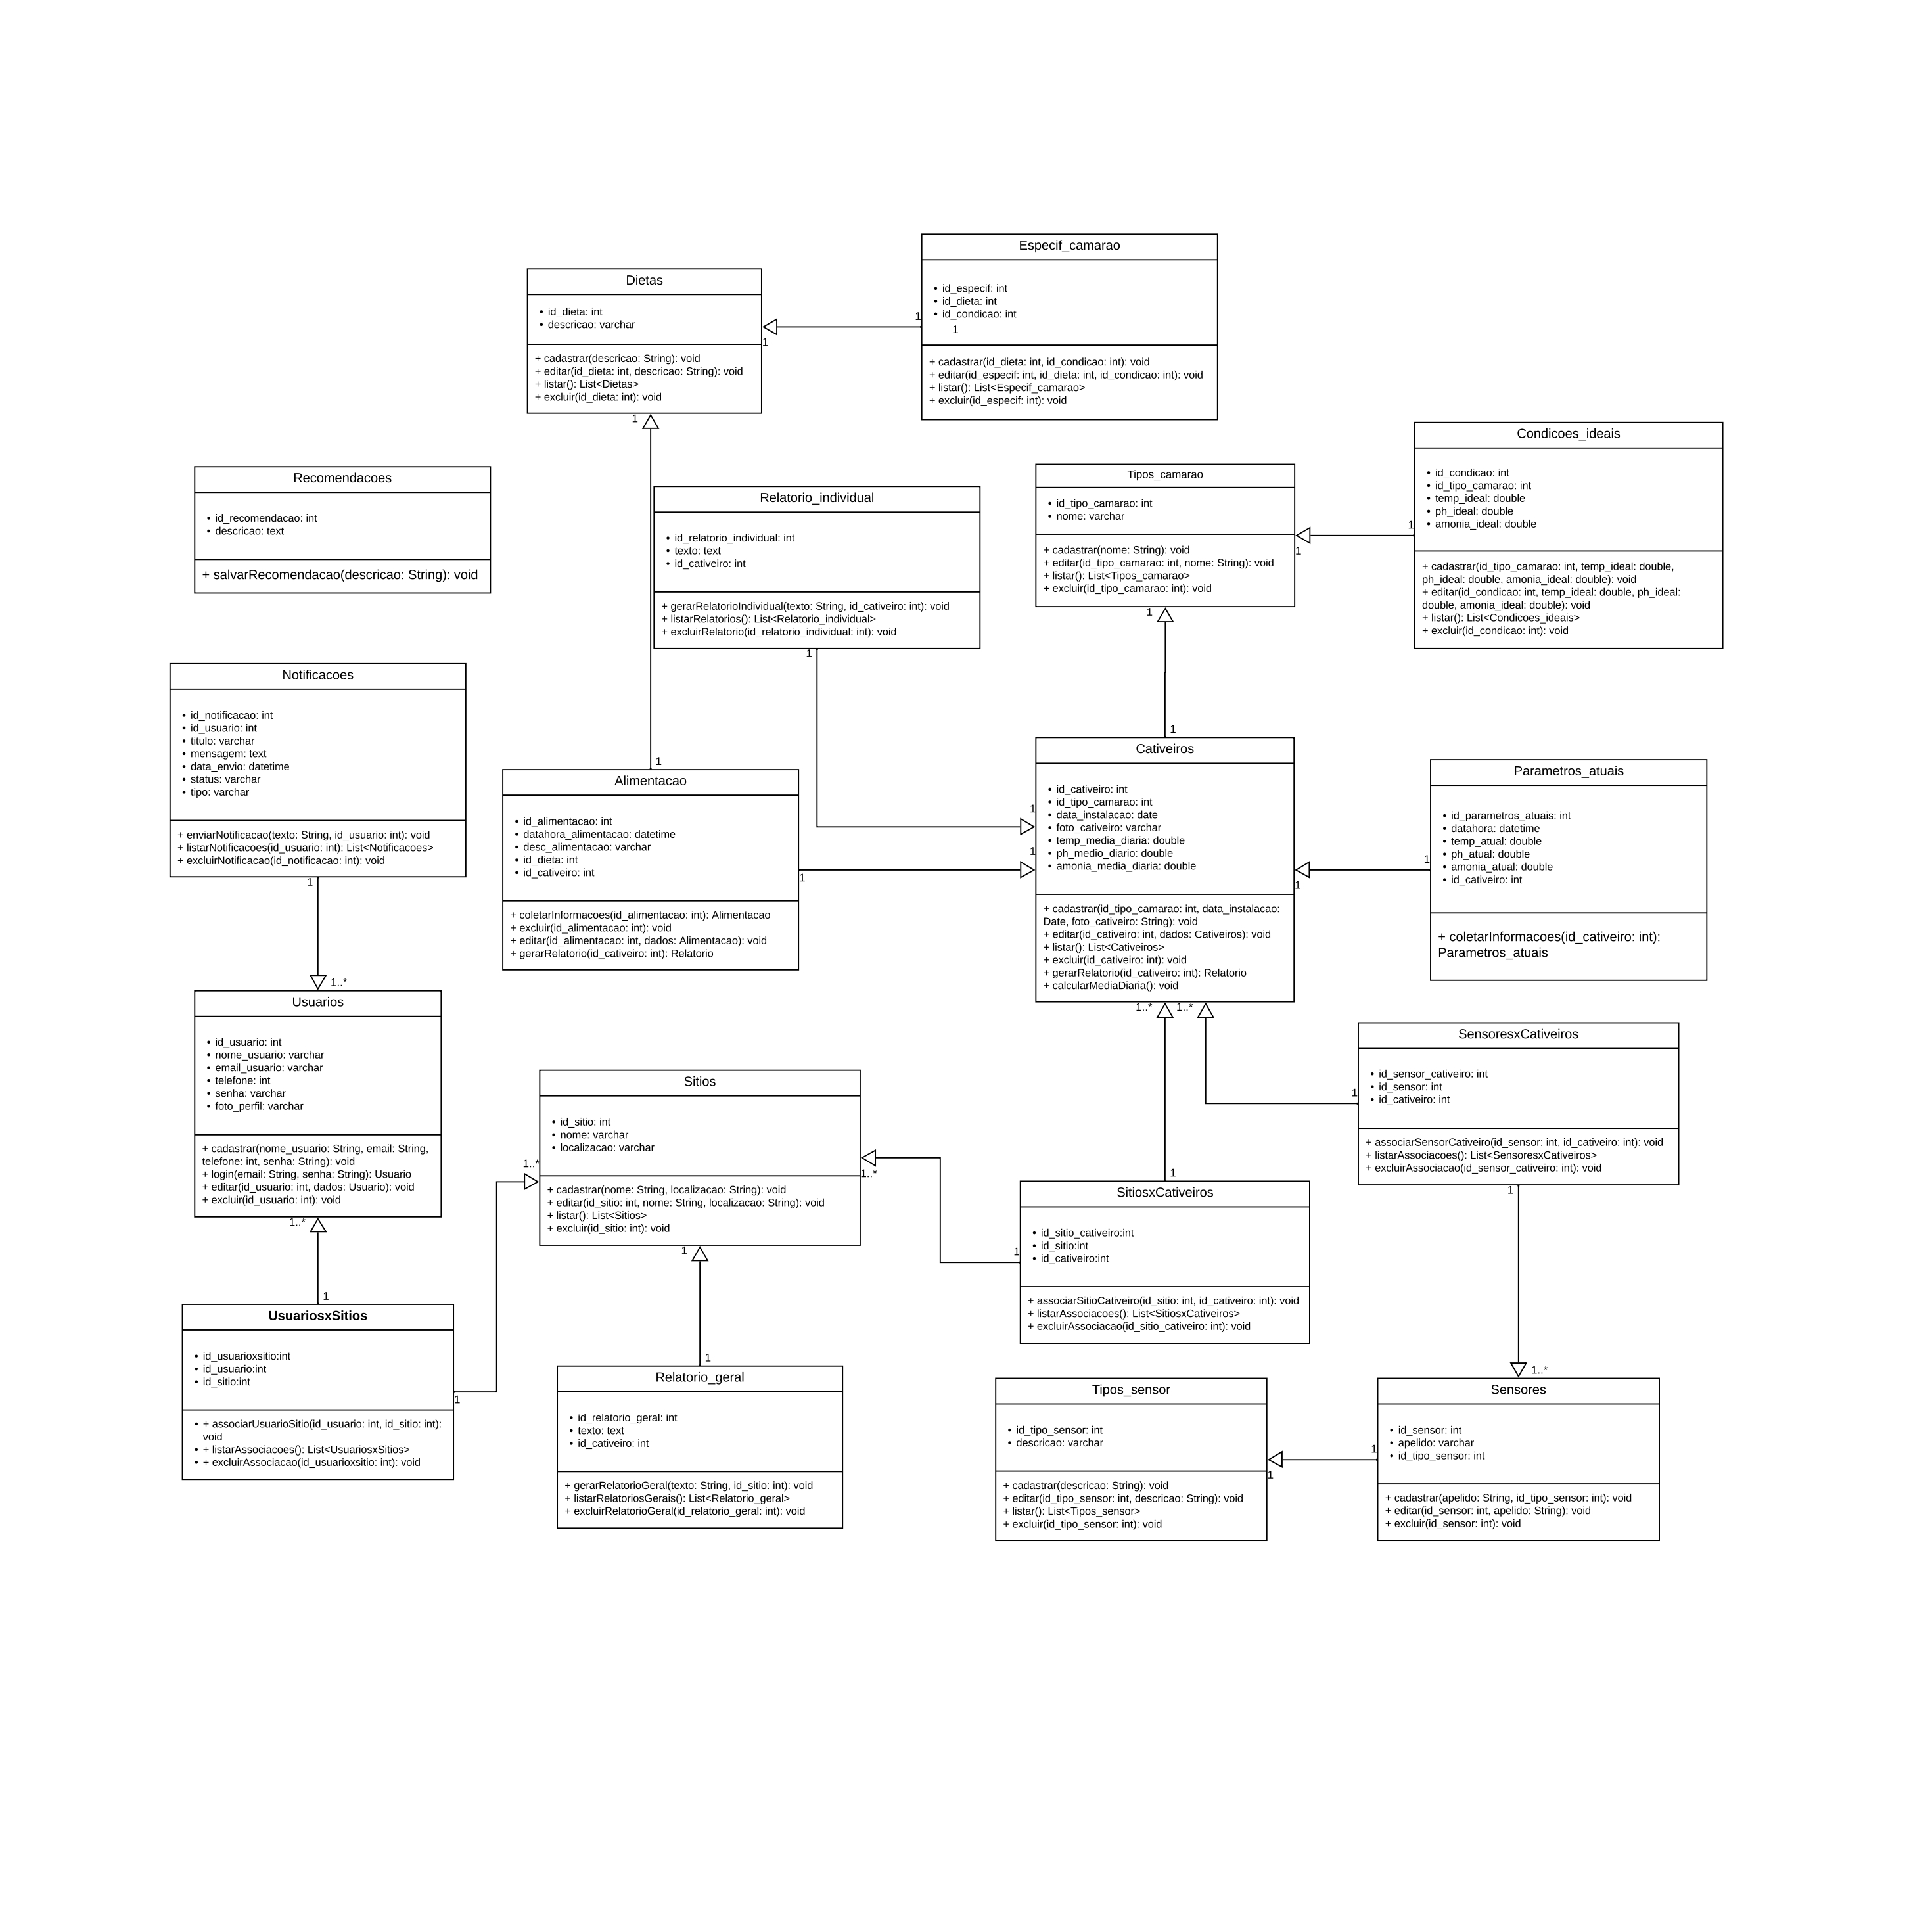
\includegraphics[width=1\textwidth]{Imagem/Diagramas de Classe.jpg}
        \SourceOrNote{Autoria Própria}
        \end{figure}

    \newpage

    \subsection*{\textbf{Diagrama de Objetos}}
    \addcontentsline{toc}{section}{Diagrama de Objetos}

O diagrama de objetos apresenta uma visão prática do sistema de gerenciamento de cativeiros, demonstrando as instâncias específicas das classes e os valores associados em um momento determinado. Ele detalha o estado de cada entidade e suas interações, facilitando a compreensão da configuração atual. 

Entre os objetos principais, temos o Sensor1, que monitora parâmetros ambientais como temperatura, pH e amônia, categorizado por TipoSensor1, que descreve seu tipo, como "Sensor de Temperatura". Esses dados são registrados em ParametrosAtuais1, com valores como temperatura de 26,8°C, pH de 8,3 e amônia de 0,02. O Cativeiro1 armazena informações detalhadas sobre o local onde os camarões, como o "Camarão Tigre" descrito por TipoCamarao1, são criados, incluindo médias diárias de parâmetros ambientais e dados de instalação. Esse cativeiro faz parte do Sitio1, chamado "Sítio de Camarões Atlântico", localizado em Registro, Brasil, que é gerenciado por um usuário, como João Pescador, representado pelo Usuario1. 

O sistema também gerencia atividades como Alimentação1, associada a uma dieta específica (Dieta1), como "Dieta Balanceada com Proteína Alta", projetada para otimizar o crescimento dos camarões. CondicoesIdeais1 define os parâmetros ambientais ideais, enquanto RelatorioGeral1 e RelatorioIndividual1 registram informações detalhadas sobre os cativeiros, fornecendo uma visão ampla ou específica para análise e gestão. Recomendacoes1 oferece sugestões práticas, como ajustes na temperatura da água, baseadas nos dados coletados. Notificação1 alerta os usuários sobre situações críticas, garantindo uma resposta rápida para manter as condições ideais. 

O diagrama demonstra como os sensores coletam dados que, integrados ao sistema, geram relatórios, notificações e recomendações para o manejo eficiente dos cativeiros, promovendo o bem-estar dos camarões criados. Ele destaca a importância das associações entre os objetos para garantir que todas as atividades e parâmetros sejam monitorados e ajustados de forma precisa.

    \begin{figure}[!h]
        \centering
        \caption{Diagrama de objetos}%
        \label{fig:diagrama-objetos}
         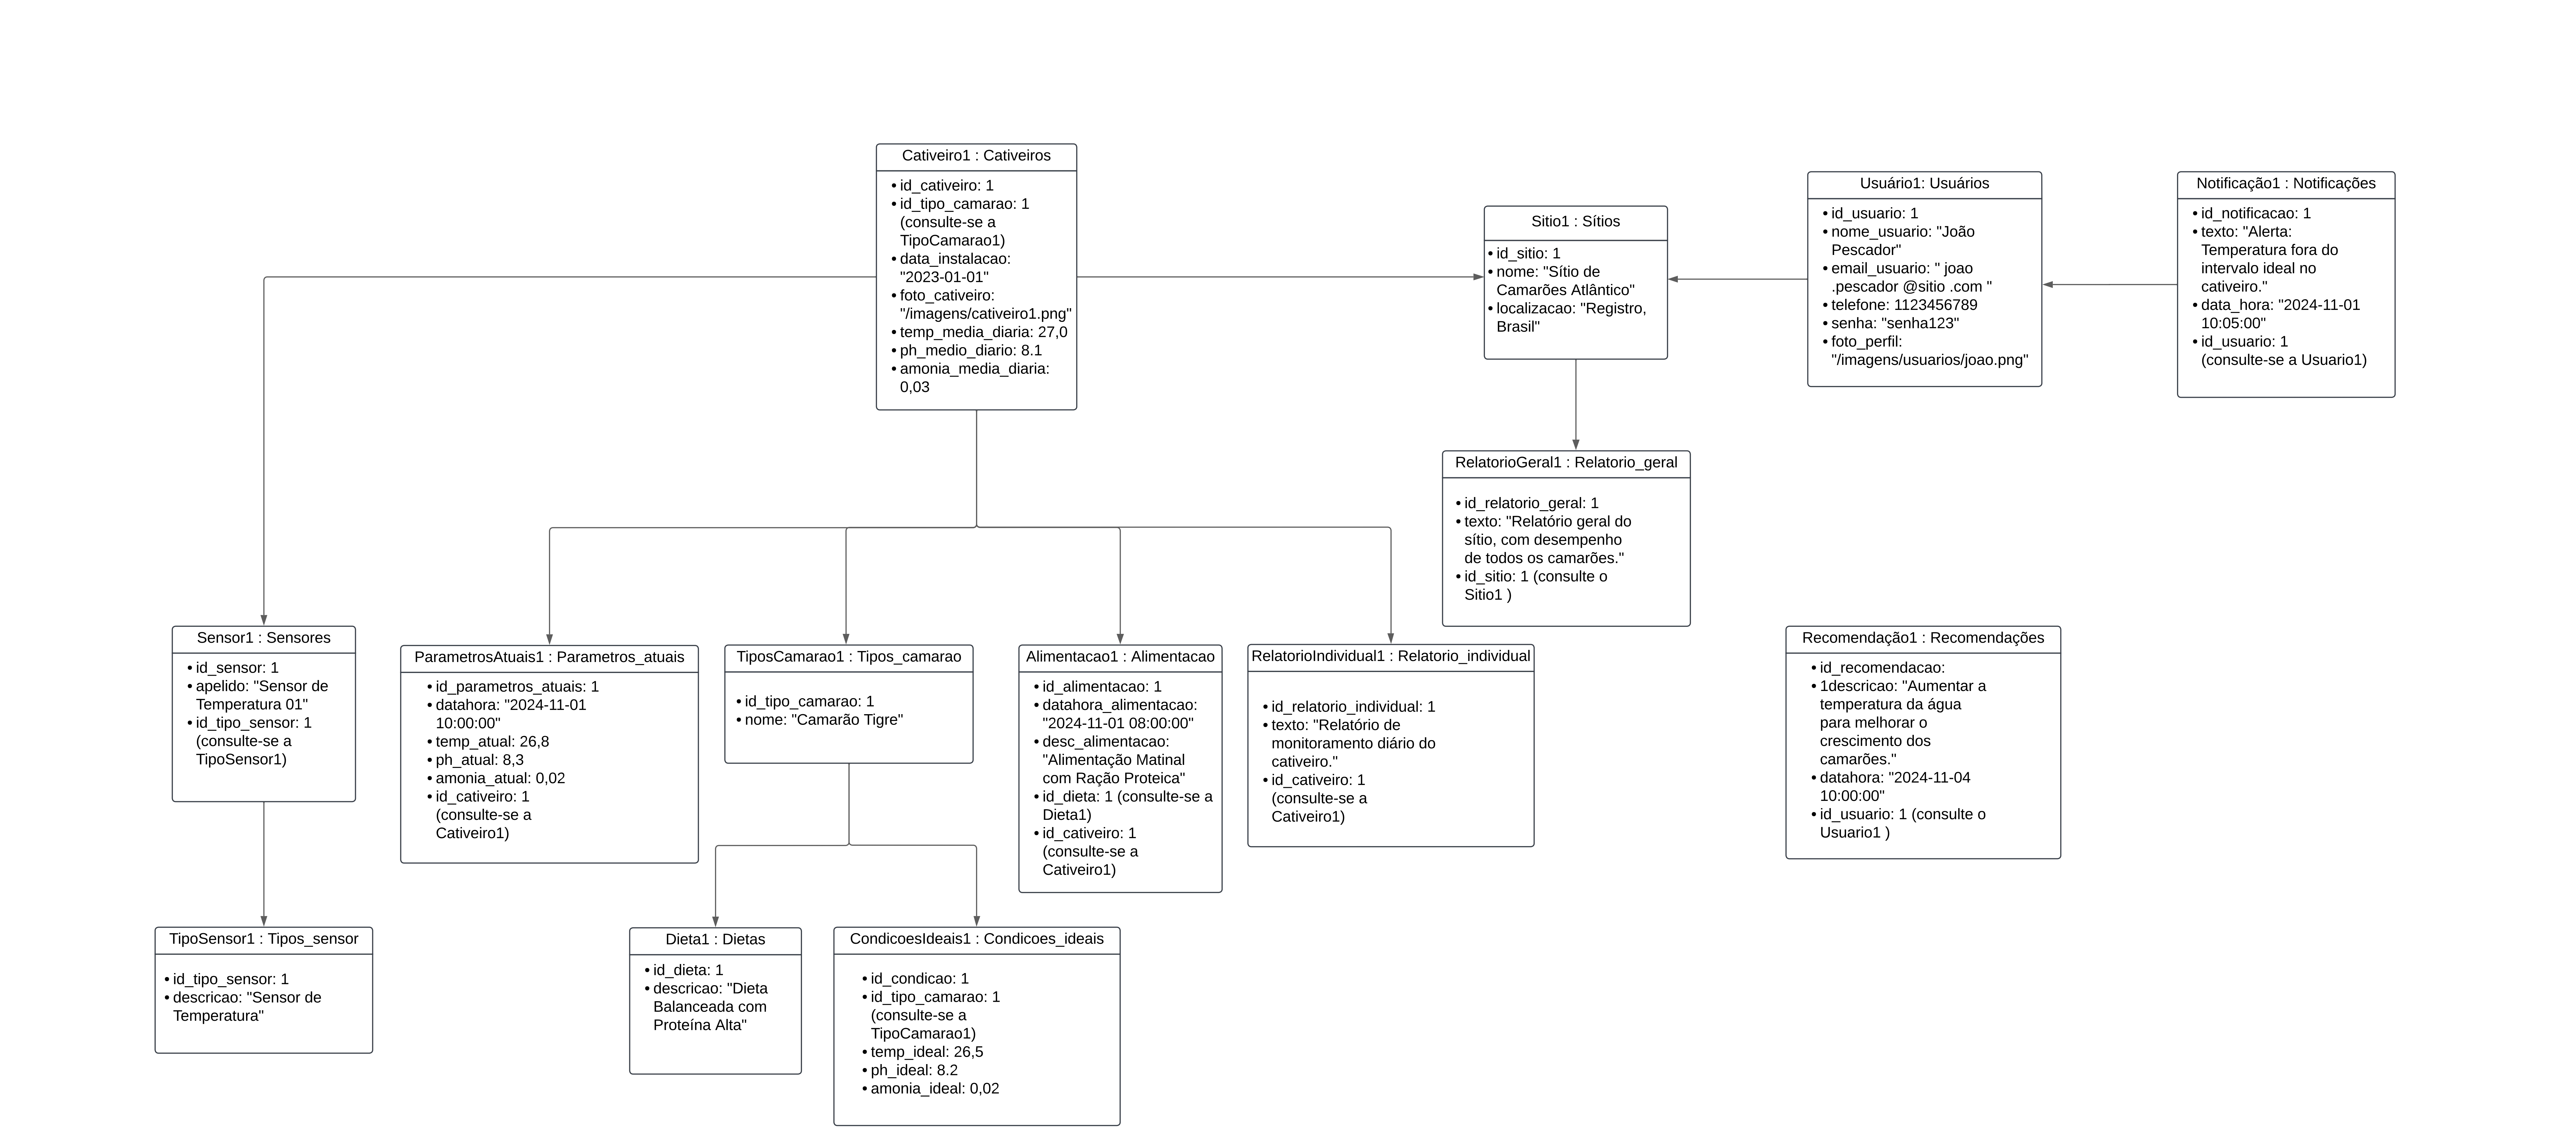
\includegraphics[width=1\textwidth]{Imagem/Diagrama de Objetos.jpg}
        \SourceOrNote{Autoria Própria}
        \end{figure}

    \newpage
       
    \subsection*{\textbf{Diagrama de Redes}}
    \addcontentsline{toc}{section}{Diagrama de Redes}

    O Diagrama de Redes foi desenvolvido com o objetivo de ilustrar o funcionamento do projeto Camarize, um Sistema de Monitoramento de Cativeiro de Camarões para Fins Gastronômicos.

    Na etapa de monitoramento, cada tanque estará equipado com um Arduino conectado a três sensores: medidor de temperatura, de pH e amônia. Que se mostram fundamentais para a avaliação da salubridade da água do cativeiro para os camarões. O dispositivo transmitirá continuamente os dados dos sensores por meio do Wi-Fi para o servidor central encontrado na sala de monitoramento.

    Na etapa de automatização da alimentação, será utilizado um dispensador de ração com uma abertura na parte inferior, equipado com um motor para controle da abertura e um sensor de nível com os parâmetros pré-definidos anteriormente para determinar a quantidade ideal de ração a ser liberada no tanque. Em que, ambos os componentes estarão conectados ao Arduino, também se comunicando via Wi-Fi com o servidor central da sala de monitoramento. Os dados serão então compartilhados com os computadores que têm acesso à plataforma.

    
\begin{figure}[h]
\centering
\caption{Diagrama de Rede}%
\label{fig:diagrama-rede}
 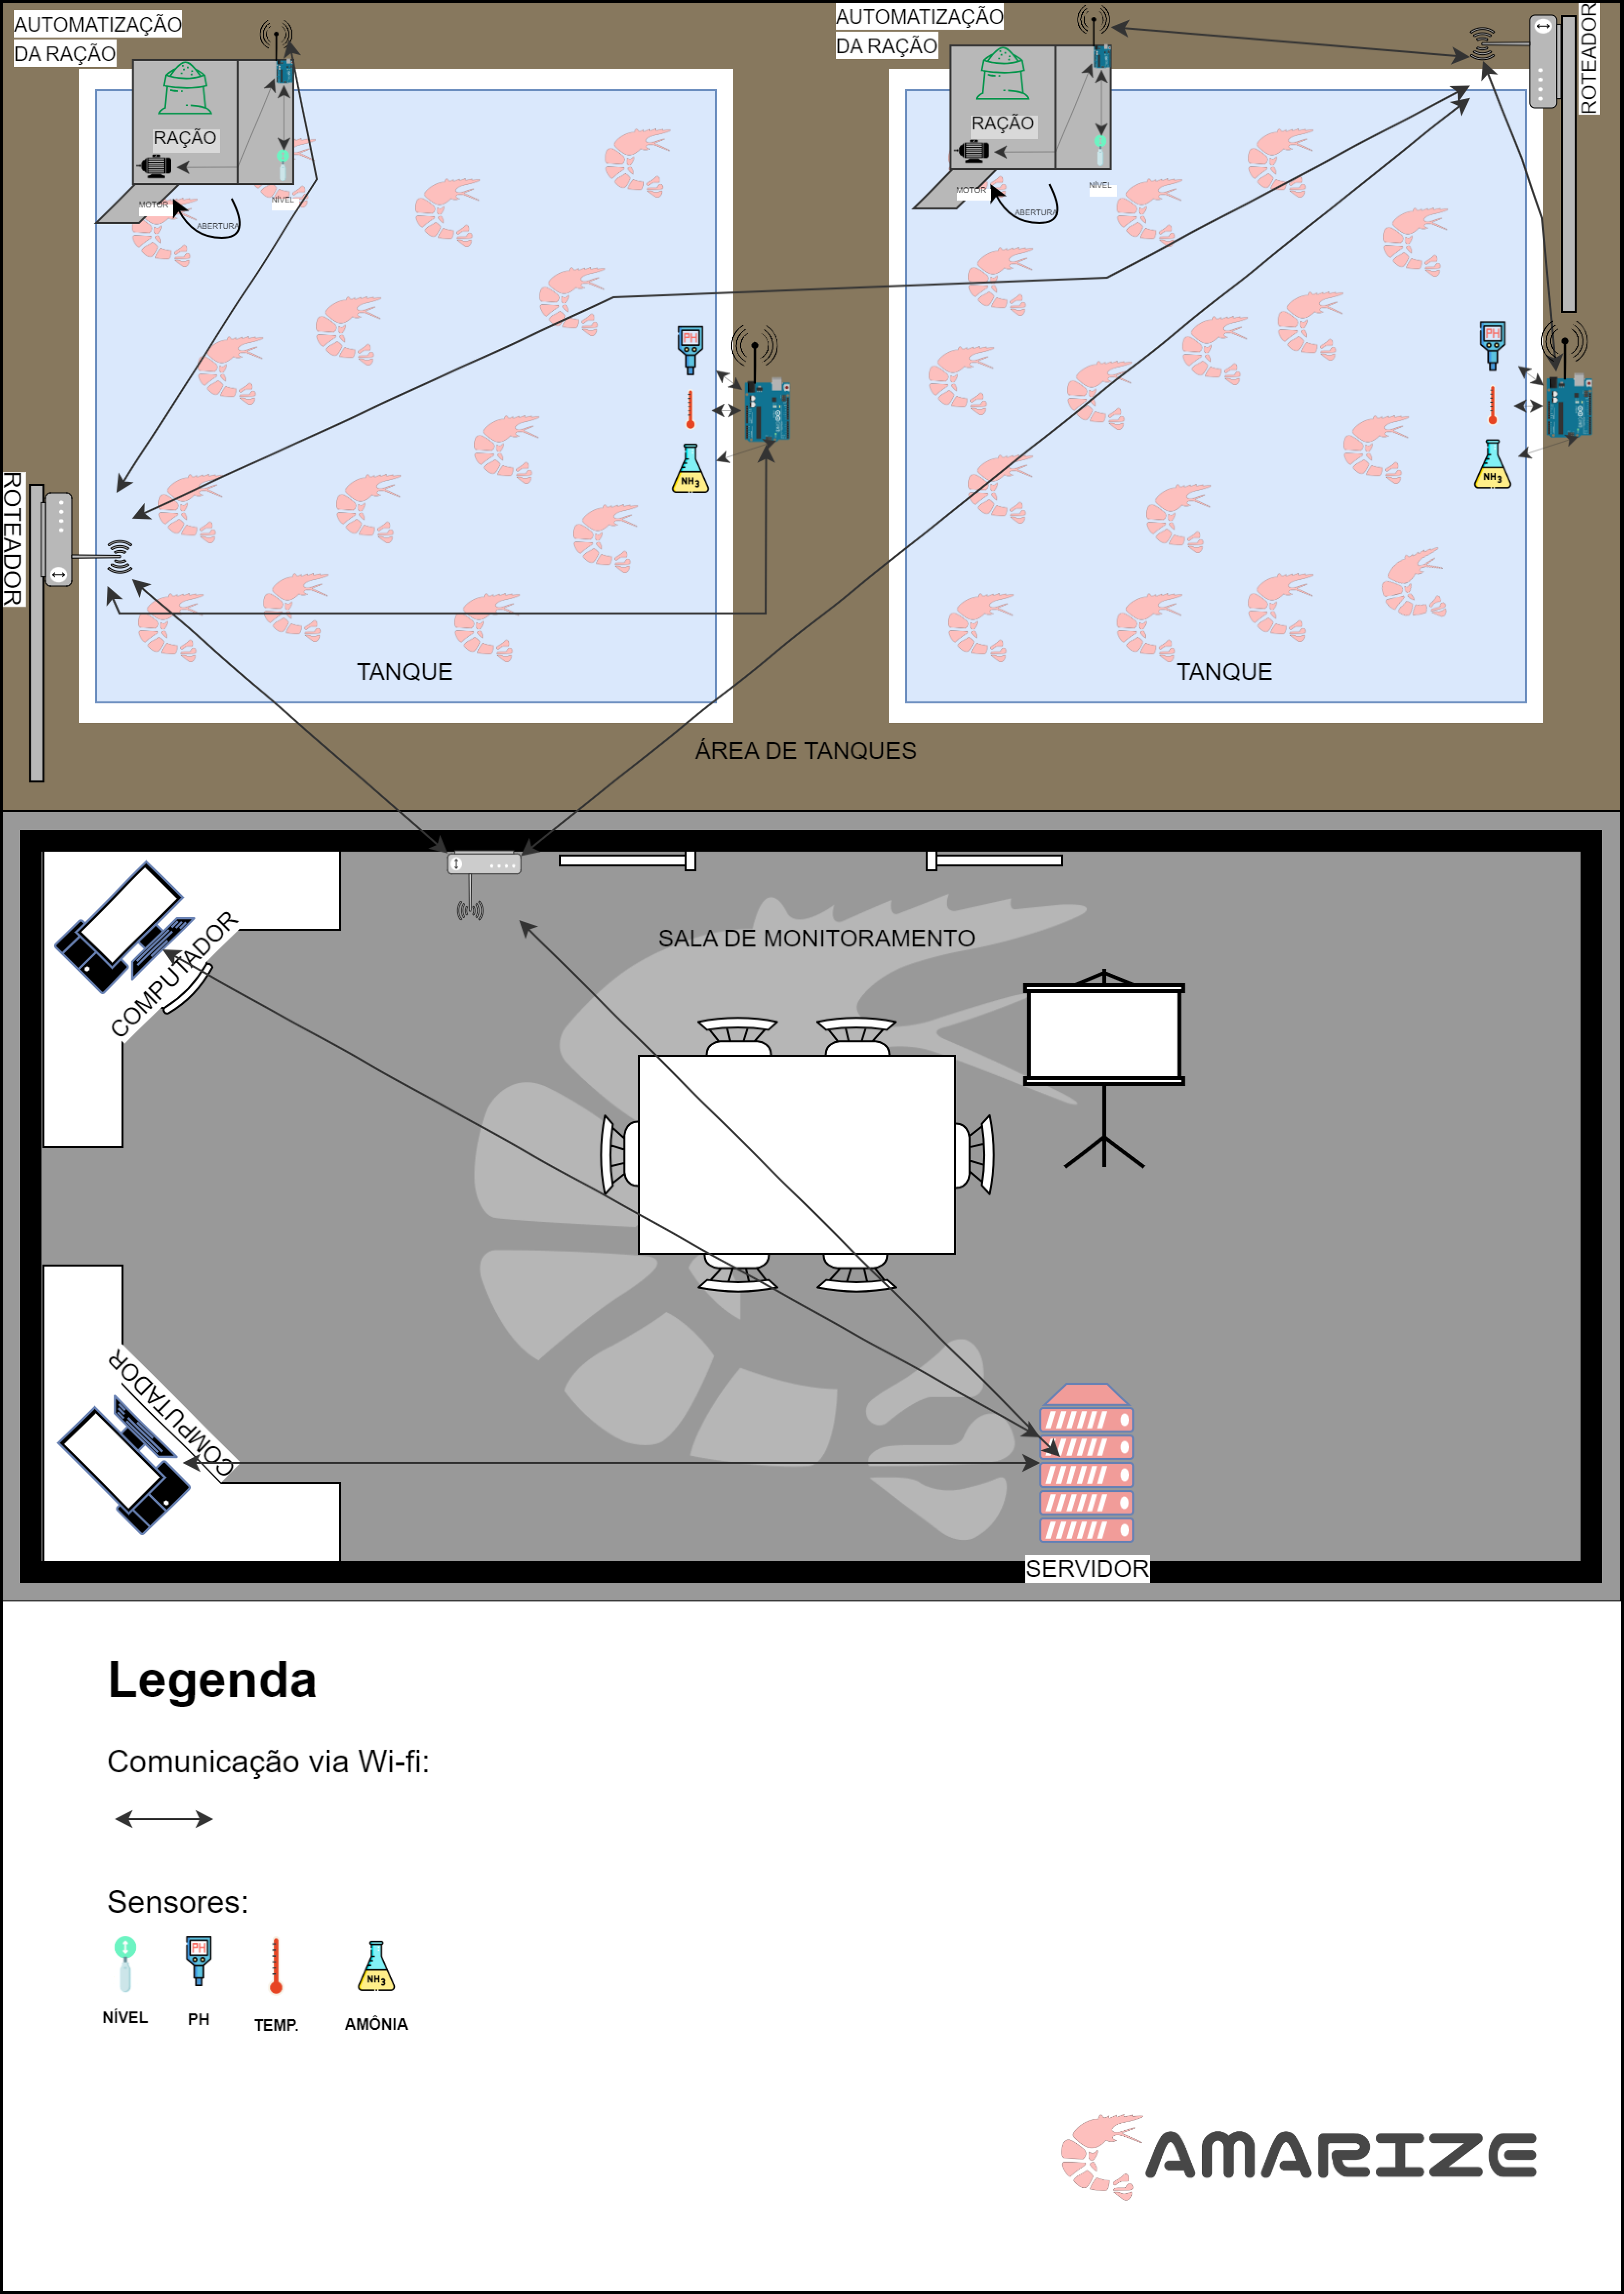
\includegraphics[width=0.6\textwidth]{Imagem/Diagrama de Redes.png}
\SourceOrNote{Autoria Própria}
\end{figure}

    \newpage

    É essencial pontuar que a comunicação entre os elementos ocorrerá via Wireless, que pode ser amplificada com uma maior quantidade de roteadores a depender da localização.

    \section*{\textbf{Modelo de Negócios Canvas}}
    \addcontentsline{toc}{section}{Modelo de Negócios Canvas}

    O modelo de negócios Canvas foi utilizado para análise econômica do sistema. Por meio do Canvas foi possível identificar os Parceiros, Recursos e Atividades Chaves, nossas Propostas de Valor, Segmento de Mercado, nossa Fonte de Renda e Estrutura de Custos.

    
\begin{figure}[h]
\centering
\caption{Canvas}%
\label{fig:canvasum}
 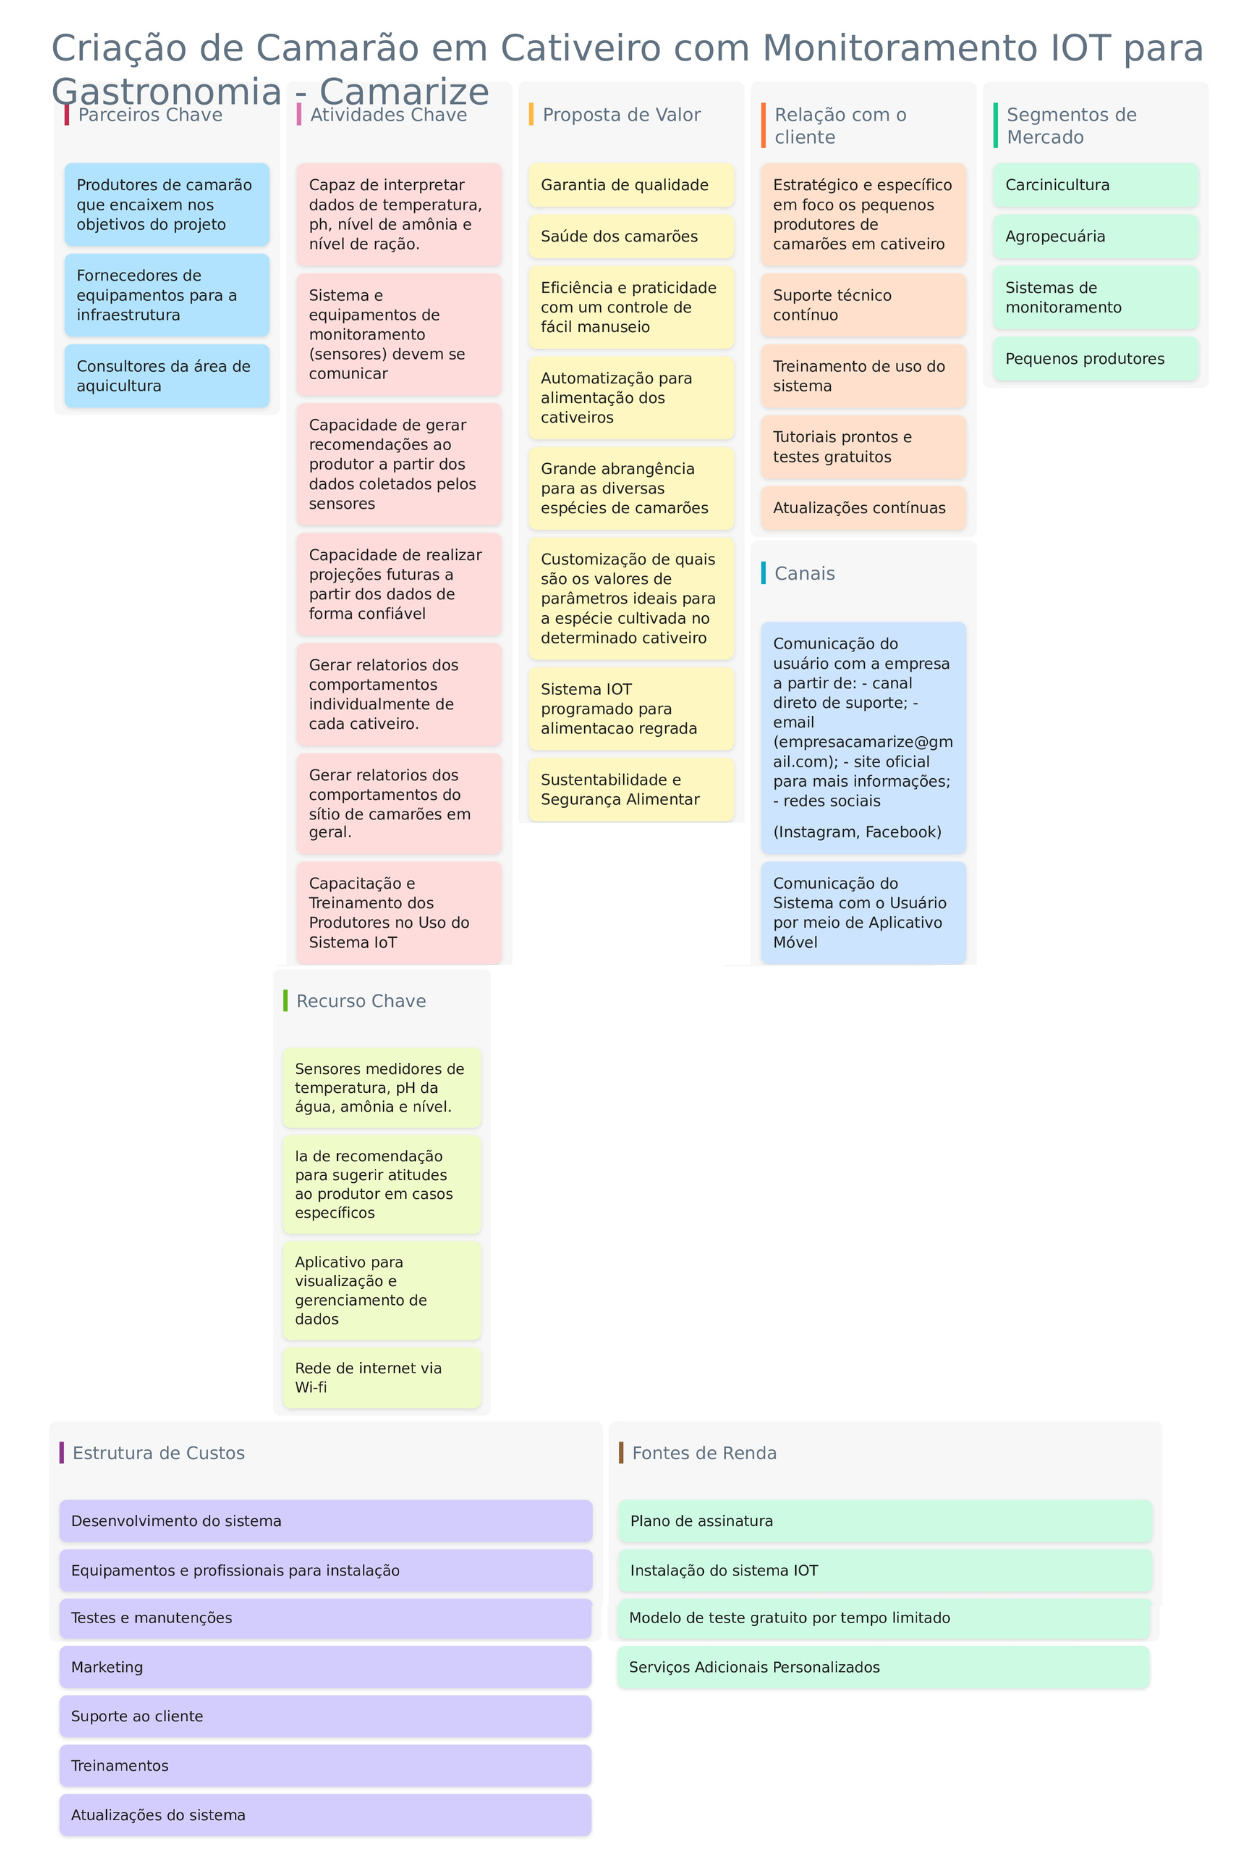
\includegraphics[width = 0.8\CaptionWidth]{Imagem/Canvas.png}
\SourceOrNote{Autoria Própria}
\end{figure}

\newpage

Foi realizada uma análise completa e incluído os possíveis dados.

\section*{\textbf{Modelo Lógico, Conceitual e Físico do Banco de Dados}}
\addcontentsline{toc}{section}{Modelo Lógico, Conceitual e Físico do Banco de Dados}

A modelagem conceitual e lógica demonstra a funcionalidade do programa e do que será aplicado no banco de dados. A visão gráfica do banco de dados se demonstra algo fundamental, por conta que proporciona o máximo de detalhes com extrema clareza, apresentando as relações entre as entidades.

No modelo conceitual, a entidade Cativeiros representa os tanques, com dados como data\_instalacao e temp\_media\_diaria. Ela está associada a Tipos\_camarao, que define a espécie criada, e a Condições\_ideais, que especifica parâmetros recomendados, como temp\_ideal e ph\_ideal.

Sensores, registrados em Sensores, monitoram os cativeiros, coletando dados armazenados em Parametros\_atuais, como temp\_atual e ph\_atual. A alimentação é controlada por Dietas e eventos específicos registrados em Alimentacao. Cativeiros estão localizados em Sitos, com atributos como nome e localizacao, e geram relatórios gerais em Relatorio\_geral.

Usuários, descritos em Usuarios, têm acesso aos dados dos cativeiros e recebem notificações e recomendações por meio das entidades Notificacoes e Recomendacoes. Os relacionamentos entre as entidades integram dados de sensores, alimentação, localização e usuários para garantir o controle eficiente do ambiente de criação.

No modelo lógico, é apresentado uma representação mais concreta do banco de dados, demonstrando as tabelas, entidades, chaves primárias e estrangeiras e seus relacionamentos.

No modelo físico, demonstra uma versão refinada do modelo conceitual, representando restrições de dados, nomes de entidades e relacionamentos para implementação de forma independente.

\newpage

\begin{figure}[!htb]
\SetCaptionWidth{\ifbool{@LayoutA}{0.7}{0.72}\linewidth}
\caption{Modelo Conceitual}%
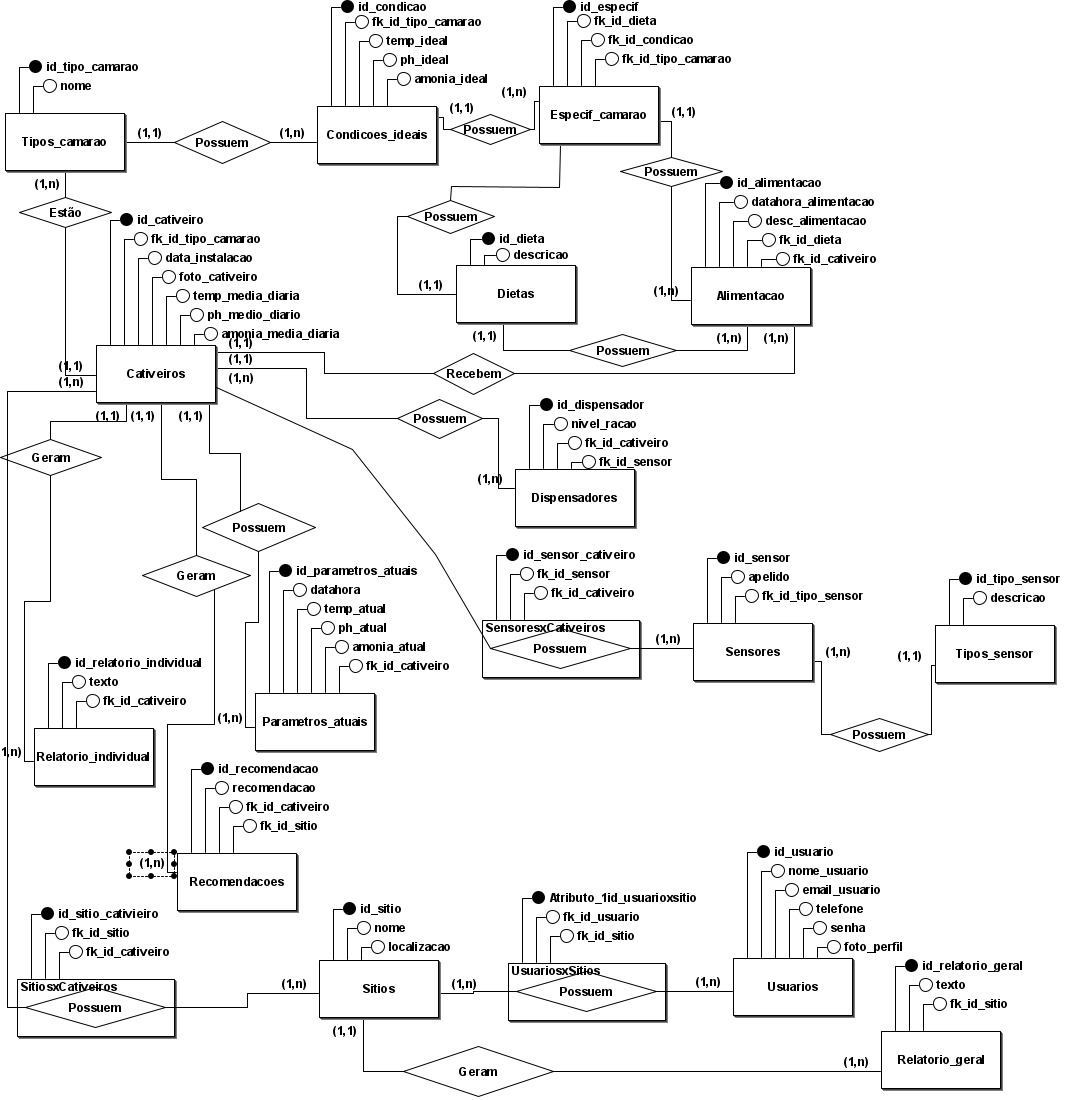
\includegraphics[width = 1.5\CaptionWidth]{Imagem/Modelo Conceitual.jpeg}
\SourceOrNote{Autoria Própria}
\end{figure}

\newpage

\begin{figure}[!htb]
\SetCaptionWidth{\ifbool{@LayoutA}{0.7}{0.72}\linewidth}
\caption{Modelo Lógico}%
\includegraphics[width = 1.5\CaptionWidth]{Imagem/Modelo Lógico.png}
\SourceOrNote{Autoria Própria}
\end{figure}

\newpage

\begin{figure}[!htb]
\SetCaptionWidth{\ifbool{@LayoutA}{0.7}{0.72}\linewidth}
\caption{Modelo Físico}%
\includegraphics[width = 1.5\CaptionWidth]{Imagem/Modelo Físico.jpg}
\SourceOrNote{Autoria Própria}
\end{figure}

O banco de dados tem um papel de extrema importância para as informações, sendo necessário para guardar, organizar e recuperar dados. O Modelo Lógico e Conceitual são maneira de demonstrar a eficiência de um banco de dados.

\newpage

\section*{\textbf{Script SQL}}
\addcontentsline{toc}{section}{Script SQL}

O Script SQL foi baseado no modelo lógico e conceitual do banco de dados. Ajuda a entender como o banco de dados deve ser montado, fazendo com que se torne algo prático. O Script conta com a criação das tabelas e se um insert into para cada uma delas.

\begin{verbatim}
    
create database camarize_bd;

use camarize_bd;
	 
# Tabela para apenas os registros dos tipos de camarão que são diversos.

create table Tipos_camarao(
	id_tipo_camarao int auto_increment primary key,
	nome varchar(100)
);
	 
# Dieta ideal.

create table Dietas(
	id_dieta int auto_increment primary key,
	descricao varchar(100)
);
	 
# Condições ideais de temperatura, pH e amônia 
# para cada tipo especifico de camarão.

create table Condicoes_ideais(
	id_condicao int auto_increment primary key,
	id_tipo_camarao int,
	temp_ideal double,
	ph_ideal double,
	amonia_ideal double,
	constraint fk_camarao_condicoes foreign key(id_tipo_camarao)
     references Tipos_camarao(id_tipo_camarao)
);

# Registro do ambiente cativeiro, relacionando com o tipo de camarão que abriga, 
# e média diária dos parâmetros.

create table Cativeiros(
	id_cativeiro int auto_increment primary key,
	id_tipo_camarao int,
	data_instalacao date,
	foto_cativeiro varchar(100),
	temp_media_diaria double,
	ph_medio_diario double,
	amonia_media_diaria double,
	constraint fk_camarao_cativeiro foreign key(id_tipo_camarao)
     references Tipos_camarao(id_tipo_camarao)
);

	 
# Parâmetros atuais de cada cativeiro.

create table Parametros_atuais(
	id_parametros_atuais int auto_increment primary key,
	datahora datetime,
	temp_atual double,
	ph_atual double,
	amonia_atual double,
	id_cativeiro int,
	constraint fk_cativeiro_parametro foreign key(id_cativeiro)
     references Cativeiros(id_cativeiro)
);
	 
# Especificação para cada tipo de camarão
# relacionando as condições ambientais ideais e dieta com o tipo de camarão.

create table Especif_camarao(
	id_especif int auto_increment primary key,
	id_dieta int,
	id_condicao int,
	constraint fk_dieta_especif foreign key(id_dieta) 
     references Dietas(id_dieta),
	constraint fk_condicao_especif foreign key(id_condicao)
     references Condicoes_ideais(id_condicao)
);
	 
	 
# Registro de alimentações dadas pelo dispensador de racão 
# de acordo com a dieta do cativeiro.

create table Alimentacao(
	id_alimentacao int auto_increment primary key,
	datahora_alimentacao datetime,
	desc_alimentacao varchar(100),
	id_dieta int,
	id_cativeiro int,
	constraint fk_dieta_alimentacao foreign key(id_dieta)
     references Dietas(id_dieta),
	constraint fk_cativeiro_alimentacao foreign key(id_cativeiro)
     references Cativeiros(id_cativeiro)
);
	 
# Registro dos sitios de camarão.

create table Sitios(
	id_sitio int auto_increment primary key,
	nome varchar(100),
	localizacao varchar(255)
);
	 
# Relacionando sitios e cativeiros.

create table SitiosxCativeiros(
	id_sitio_cativieiro int auto_increment primary key,
	id_sitio int,
	id_cativeiro int,
	constraint fk_sitio_sitioxcat foreign key(id_sitio)
     references Sitios(id_sitio),
	constraint fk_cativeiro_sitioxcat foreign key(id_cativeiro)
     references Cativeiros(id_cativeiro)
);
	 
# Conta de usuário.

create table Usuarios(
	id_usuario int auto_increment primary key,
	nome_usuario varchar(100),
	email_usuario varchar(50),
	telefone varchar(11),
	senha varchar(50),
	foto_perfil varchar(100)
);
	 
# Relacionando cada usuário com seu sitio.

create table UsuariosxSitios(
	id_usuarioxsitio int auto_increment	primary key,
	id_usuario int,
	id_sitio int,
	constraint fk_usuario_usuxsitio foreign key(id_usuario)
     references Usuarios(id_usuario),
	constraint fk_sitio_usuxsitio foreign key(id_sitio)
     references Sitios(id_sitio)
);
	 
# Criar registros de relatórios de tanques individuais. 

create table Relatorio_individual(
	id_relatiorio_individual int auto_increment primary key,
	texto text,
	id_cativeiro int,
	constraint fk_cativeiro_relatorio_i foreign key(id_cativeiro)
     references Cativeiros(id_cativeiro)
);
	 
# Criar registros de relatórios de todos os tanques do sitio.

create table Relatorio_geral(
	id_relatorio_geral int auto_increment primary key,
	texto text,
	id_cativeiro int,
	id_sitio int,
	constraint fk_sitio_relatorio_g foreign key(id_sitio)
     references Sitios(id_sitio)
);
	 
# Tipos de sensor.

create table Tipos_sensor(
	id_tipo_sensor int auto_increment primary key,
	descricao varchar(50)
);
	 
# Registrar sensor.

create table Sensores(
	id_sensor int auto_increment primary key,
	apelido varchar(100),
	id_tipo_sensor int,
	constraint fk_tipo_sensores foreign key(id_tipo_sensor)
     references Tipos_sensor(id_tipo_sensor)
);
	 
# Relacionando quais sensores estão presentes em quais cativeiros.

create table SensoresxCativeiros(
	id_sensor_cativeiro int auto_increment primary key,
	id_sensor int,
	id_cativeiro int,
	constraint fk_sensor_cativeiros foreign key(id_sensor)
     references Sensores(id_sensor),
	constraint fk_cativeiro_sensor foreign key(id_cativeiro)
     references Cativeiros(id_cativeiro)
);
	 
# Recomendações a serem feitas.

create table Recomendacoes(
	id_recomendacao int auto_increment primary key,
	recomendacao text,
	id_cativeiro int,
	id_sitio int,
	constraint fk_cativeiro_rec foreign key(id_cativeiro)
     references Cativeiros(id_cativeiro),
	constraint fk_sitio_rec foreign key(id_sitio)
     references Sitios(id_sitio)
);
    
# Tipos_camarao

insert into Tipos_camarao (nome) values ('Camarão Branco');
insert into Tipos_camarao (nome) values ('Camarão Rosa');
insert into Tipos_camarao (nome) values ('Camarão Tigre');

# Dietas

insert into Dietas (descricao) values ('Dieta Proteica');
insert into Dietas (descricao) values ('Dieta Equilibrada');
insert into Dietas (descricao) values ('Dieta Vegetariana');

# Condicoes_ideais

insert into Condicoes_ideais (id_tipo_camarao, temp_ideal, ph_ideal, amonia_ideal) 
values (1, 27.5, 7.8, 0.1);
insert into Condicoes_ideais (id_tipo_camarao, temp_ideal, ph_ideal, amonia_ideal) 
values (2, 25.0, 7.5, 0.2);
insert into Condicoes_ideais (id_tipo_camarao, temp_ideal, ph_ideal, amonia_ideal) 
values (3, 28.0, 7.9, 0.15);

# Cativeiros

insert into Cativeiros (id_tipo_camarao, data_instalacao, foto_cativeiro,
 temp_media_diaria, ph_medio_diario, amonia_media_diaria) 
values (1, '2024-01-10', 'foto1.jpg', 26.8, 7.7, 0.1);
insert into Cativeiros (id_tipo_camarao, data_instalacao, foto_cativeiro,
 temp_media_diaria, ph_medio_diario, amonia_media_diaria) 
values (2, '2024-02-15', 'foto2.jpg', 25.2, 7.5, 0.2);
insert into Cativeiros (id_tipo_camarao, data_instalacao, foto_cativeiro,
 temp_media_diaria, ph_medio_diario, amonia_media_diaria) 
values (3, '2024-03-20', 'foto3.jpg', 28.1, 7.9, 0.15);

# Parametros_atuais

insert into Parametros_atuais (datahora, temp_atual, ph_atual,
 amonia_atual, id_cativeiro) 
values ('2024-11-15 08:00:00', 27.0, 7.8, 0.1, 1);
insert into Parametros_atuais (datahora, temp_atual, ph_atual,
 amonia_atual, id_cativeiro) 
values ('2024-11-15 09:00:00', 25.1, 7.5, 0.2, 2);
insert into Parametros_atuais (datahora, temp_atual, ph_atual,
 amonia_atual, id_cativeiro) 
values ('2024-11-15 10:00:00', 28.0, 7.9, 0.15, 3);

# Especif_camarao

insert into Especif_camarao (id_dieta, id_condicao) values (1, 1);
insert into Especif_camarao (id_dieta, id_condicao) values (2, 2);
insert into Especif_camarao (id_dieta, id_condicao) values (3, 3);

# Alimentacao

insert into Alimentacao (datahora_alimentacao, desc_alimentacao,
 id_dieta, id_cativeiro) 
values ('2024-11-15 08:30:00', 'Ração Proteica', 1, 1);
insert into Alimentacao (datahora_alimentacao, desc_alimentacao,
 id_dieta, id_cativeiro) 
values ('2024-11-15 09:00:00', 'Ração Equilibrada', 2, 2);
insert into Alimentacao (datahora_alimentacao, desc_alimentacao,
 id_dieta, id_cativeiro) 
values ('2024-11-15 10:30:00', 'Ração Vegetariana', 3, 3);

# Sitios

insert into Sitios (nome, localizacao) values ('Sítio do Camarão 1', 'Local A');
insert into Sitios (nome, localizacao) values ('Sítio do Camarão 2', 'Local B');
insert into Sitios (nome, localizacao) values ('Sítio do Camarão 3', 'Local C');

# SitiosxCativeiros

insert into SitiosxCativeiros (id_sitio, id_cativeiro) values (1, 1);
insert into SitiosxCativeiros (id_sitio, id_cativeiro) values (2, 2);
insert into SitiosxCativeiros (id_sitio, id_cativeiro) values (3, 3);

# Usuarios

insert into Usuarios (nome_usuario, email_usuario, telefone, senha, foto_perfil) 
values ('João Silva', 'joao@example.com', '12345678901', 'senha123', 'joao.jpg');
insert into Usuarios (nome_usuario, email_usuario, telefone, senha, foto_perfil) 
values ('Maria Santos', 'maria@example.com', '98765432109', 'senha456', 'maria.jpg');
insert into Usuarios (nome_usuario, email_usuario, telefone, senha, foto_perfil) 
values ('Pedro Almeida', 'pedro@example.com', '11223344556', 'senha789', 'pedro.jpg');

# UsuariosxSitios

insert into UsuariosxSitios (id_usuario, id_sitio) values (1, 1);
insert into UsuariosxSitios (id_usuario, id_sitio) values (2, 2);
insert into UsuariosxSitios (id_usuario, id_sitio) values (3, 3);

# Relatorio_individual

insert into Relatorio_individual (texto, id_cativeiro) 
values ('Parâmetros dentro do ideal.', 1);
insert into Relatorio_individual (texto, id_cativeiro) 
values ('pH levemente elevado.', 2);
insert into Relatorio_individual (texto, id_cativeiro) 
values ('Temperatura ideal.', 3);

# Relatorio_geral

insert into Relatorio_geral (texto, id_cativeiro, id_sitio)
values ('Todos os tanques estão estáveis.', 1, 1);
insert into Relatorio_geral (texto, id_cativeiro, id_sitio) 
values ('Necessário ajustar pH em alguns tanques.', 2, 2);
insert into Relatorio_geral (texto, id_cativeiro, id_sitio) 
values ('Temperaturas em níveis ideais.', 3, 3);

# Tipos_sensor

insert into Tipos_sensor (descricao) values ('Sensor de Temperatura');
insert into Tipos_sensor (descricao) values ('Sensor de pH');
insert into Tipos_sensor (descricao) values ('Sensor de Amônia');

# Sensores

insert into SensoresxCativeiros (id_sensor, id_cativeiro) values (1, 1);
insert into SensoresxCativeiros (id_sensor, id_cativeiro) values (2, 2);
insert into SensoresxCativeiros (id_sensor, id_cativeiro) values (3, 3);

# Recomendacoes

insert into Recomendacoes (recomendacao, id_cativeiro, id_sitio) 
values ('Ajustar temperatura para o ideal.', 1, 1);
insert into Recomendacoes (recomendacao, id_cativeiro, id_sitio) 
values ('Reduzir amônia para níveis aceitáveis.', 2, 2);
insert into Recomendacoes (recomendacao, id_cativeiro, id_sitio) 
values ('Manter os parâmetros estáveis.', 3, 3);

\end{verbatim}

\section*{\textbf{Análise de recorrência do algoritmo Merge Sort}}
\addcontentsline{toc}{section}{Análise de recorrência do algoritmo Merge Sort}

O Merge Sort é um algoritmo de ordenação que consiste em dividir uma estrutura de subconjuntos e aplicar a ordenação nos elementos que são extraídos da estrutura primária. Após a ordenação dos subconjuntos, é realizada a mistura para um conjunto final ordenado.

O melhor tempo ocorre quando todos os elementos do array já estão ordenados, o Merge Sort sempre executa a divisão e a fusão, independente  da ordem dos elementos. O tempo de execução, representado por \( O(n \log_2 n) \), pode ser explicado da seguinte forma: \( \log_2 n \) corresponde ao número de divisões do array até que cada subarray contenha apenas um elemento, e \( n \) refere-se ao número de comparações e fusões realizadas durante o processo de merge.

O tempo médio ocorre quando os elementos estão em ordens aleatórias, em seu comportamento o número de divisões e fusões não dependem da ordem dos elementos, cada nível realiza \( n \) operações no total e possui \( \log_2 n \) níveis. Sua representação é semelhante com o melhor tempo: \( O(n \log_2 n) \).

O pior tempo ocorre quando o array está em ordem oposta a esperada, sua complexidade não é alterada por conta que sua quantidade de execuções não são alteradas. Sua representação se mantém a mesma, sendo ela: \( \log_2 n \).

Na aplicação, foi utilizada na tela de sensores, sendo utilizado para organizar os sensores de forma crescente e decrescente. Seu tempo de execução foram exatos 0.000000 milisegundos, mostrando a eficiência e rapidez do algoritmo. Sua representação matemática se apresenta desta maneira:

\[
\text{MergeSort}(n) =
\begin{cases}
0, & \text{se } n = 0 \\
0, & \text{se } n = 1 \\
2 \cdot \text{MergeSort}\left(\frac{n}{2}\right) + O(n), & \text{se } n > 1
\end{cases}
\]

\textbf {A representação do código:} 

\begin{verbatim}
    
function mergeSort(arr) {
    if (arr.length <= 1) return arr;

    const mid = Math.floor(arr.length / 2);
    const left = mergeSort(arr.slice(0, mid));
    const right = mergeSort(arr.slice(mid));

    return merge(left, right);
    }

    function merge(left, right) {
        let result = [], leftIndex = 0, rightIndex = 0;

    while (leftIndex < left.length && rightIndex < right.length) {
        if (left[leftIndex].id_tipo_sensor > right[rightIndex].id_tipo_sensor) {
            result.push(left[leftIndex]);
            leftIndex++;
        } else {
            result.push(right[rightIndex]);
            rightIndex++;
        }
    }

    return result.concat(left.slice(leftIndex), right.slice(rightIndex));
}

\end{verbatim}

\textbf {A representação em pseudocódigo:} 

\begin{verbatim}

funcao mergeSort(arr[])

    // Função recursiva para ordenar o vetor usando o algoritmo MergeSort

    se tamanho de arr <= 1 então
        retornar arr
    fimse

    meio <- arredondar_para_baixo(arr.length / 2)
    esquerda <- mergeSort(arr[0, meio])
    direita <- mergeSort(arr[meio, arr.length])

    retornar merge(esquerda, direita)
fimfuncao

funcao merge(esquerda[], direita[])

    // Função para combinar dois vetores ordenados

    resultado <- lista_vazia
    indice_esquerda <- 0
    indice_direita <- 0

    enquanto indice_esquerda < tamanho de esquerda e 
    indice_direita < tamanho de direita faça
    se 
    esquerda[indice_esquerda].id_tipo_sensor > direita[indice_direita].id_tipo_sensor 
        então
            adicionar esquerda[indice_esquerda] em resultado
            indice_esquerda incrementa 1
        senão
            adicionar direita[indice_direita] em resultado
            indice_direita incrementa 1
        fimse
    fimenquanto

    retornar resultado concatenado com esquerda[indice_esquerda, arr.length] 
    e direita[indice_direita, arr.length]
fimfuncao

\end{verbatim}



\section*{\textbf{Diário de Bordo}}
\addcontentsline{toc}{section}{Diário de Bordo}
\includepdf[pages={2,3,4,5}]{Imagem/Diário de Bordo - Criação de Camarão em Cativeiro Com Monitoramento IOT Para Gastronomia.pdf}
    
\end{document}